\documentclass[onecolumn]{emulateapj}
\newcommand{\beq}{\begin{equation}}
\newcommand{\eeq}{\end{equation}}
\newcommand{\hyd}    {{\rm H}}
\newcommand{\vobs}{v_{\rm obs}}
\newcommand{\hi}{H{\sc i}~}
\newcommand{\hii}{H{\sc ii}~}
\newcommand{\hia}{H{\sc i}}
\newcommand{\hiia}{H{\sc ii}}

\usepackage[colorlinks,urlcolor=blue,citecolor=blue,linkcolor=blue]{hyperref}
\usepackage{gensymb}
\usepackage{amsmath}
\usepackage{color}
%\usepackage{appendix}
\usepackage[titletoc,title]{appendix}
\usepackage{cleveref}


\makeatletter
\setlength{\@fptop}{0pt}
\setlength{\@fpbot}{0pt}
\setlength{\@fpsep}{0pt}
\makeatother

\newcommand{\citei}[1]{\citeauthor{#1} \citeyear{#1}}
\newcommand{\unit}[1]{\textrm{ #1}}
\newcommand{\kms}{km ${\rm s^{-1}}$}
\newcommand{\kmsa}{km ${\rm s^{-1}}$}
\newcommand{\citeia}[2]{\citeauthor{#1}~(\citeyear{#1};~#2)}

\newcommand\reye{\mathrm{Re}}
\newcommand\reym{\mathrm{Rm}}

\newcommand{\uphi}{\ensuremath{u_\phi}}
\newcommand{\rhat}{\ensuremath{\mathbf{\hat{r}}}}
\newcommand{\phihat}{\ensuremath{\mathbf{\hat{\phi}}}}
\newcommand{\zhat}{\ensuremath{\mathbf{\hat{z}}}}
\newcommand{\xhat}{\ensuremath{\mathbf{\hat{x}}}}
\newcommand{\yhat}{\ensuremath{\mathbf{\hat{y}}}}

\renewcommand{\topfraction}{0.85}
\renewcommand{\textfraction}{0.1}
\renewcommand{\floatpagefraction}{0.75}

\begin{document}

\title{The Weakly Nonlinear Standard and Helical Magnetorotational Instabilities in a Taylor Couette Flow}
\author{Clark, S.E.\altaffilmark{1}}
\author{Oishi, J.S. \altaffilmark{2,}\altaffilmark{3}}
%\author{Mac Low, M.-M.\altaffilmark{1,}\altaffilmark{2}}
\altaffiltext{1}{Department of Astronomy, Columbia University, New York, NY} 
\altaffiltext{2}{Department of Astrophysics, American Museum of Natural History, New York, NY}
\altaffiltext{3}{Department of Physics, SUNY Farmingdale}


\begin{abstract}
Wide gap formulation and preliminary results
\end{abstract}

\section{Introduction}

The magnetorotational instability (MRI) is thought to be a crucial driver of angular momentum transport and turbulence in astrophysical disks. (more MRI intro)

%The MRI is fundamental to our understanding of star formation, but its 
- people make a number of simplifications, incl thin gap, shearing box, etc

Despite the challenges inherent in studying the MRI, much progress has been made nu

Because of the MRI's complexity, analytical treatments of the MRI use some combination of convenient approximations: ideal MHD, linearized equations, expedient boundary conditions, and simplified geometries. In particular, much of the analytical work on MRI saturation has focused on local approximations, often representing a section of a disk by solving the MHD equations in an isolated region subject to shear periodic boundary conditions (the ``shearing box"). While the MRI is a local instability, 

Many investigations of the MRI use the ``narrow gap" approximation, in which the radial extent of the fluid channel is taken to be much smaller than the radius of curvature. That is, for a channel center $r_0$ bounded by inner and outer radii $r_1$ and $r_2$, respectively, the narrow gap approximation applies when $r_0 \gg (r_2 - r_1)$. The narrow gap approximation simplifies the MRI equations by excluding curvature terms, because the flow through a narrow gap can be taken to be approximately linear in $\phi$, i.e. Cartesian. Previous investigations into the weakly nonlinear MRI have used this narrow gap approximation (\citei{Umurhan:2007dz}, \citei{Umurhan:2007hs}, \citei{Clark:2016}). In this work we undertake the first (to our knowledge) weakly nonlinear analysis of the MRI in the wide gap regime, where the channel width may be comparable to or larger than its distance from the center of rotation.

Because we include curvature terms, our theory is also relevant to the helical magnetorotational instability (HMRI). Discovered by \citeauthor{Hollerbach:2005tr} (\citeyear{Hollerbach:2005tr}), the HMRI is an overstability in which the background magnetic field is helical. The HMRI currently occupies a special place in the MRI puzzle. The HMRI has been proposed as a method of awakening angular momentum transport in the ``dead zones" of protoplanetary disks where the magnetic Prandtl number ($Pm = \nu/\eta$) becomes very small. However the rotation profiles needed to excite HMRI may be prohibitively steeper than Keplerian depending on the boundary conditions, and so its role in astrophysical disks is currently debated (\citei{Liu:2006}, \citei{Rudiger:2007}, \citei{Kirillov:2013}). However, the HMRI is significantly easier to excite in a laboratory setting than the standard MRI, and has already been detected in the laboratory by the Potsdam Rossendorf Magnetic Instability Experiment (PROMISE; \citei{Stefani:2006iv}, \citei{Stefani:2009hp}).

We explore the weakly nonlinear HMRI

\section{Wide Gap Equations}

The basic equations solved are the momentum and induction equations,

\beq\label{momentum}
%\begin{split}
\partial_t \mathbf{u} + \mathbf{u} \cdot \nabla \mathbf{u} = -\frac{1}{\rho}\nabla P - \nabla\Phi + \frac{1}{\rho} \left(\mathbf{J}\times\mathbf{B}\right) + \nu\nabla^2 \mathbf{u} 
%\end{split}
\eeq

and

\beq\label{induction}
\partial_t \mathbf{B} = \nabla \times \left(\mathbf{u} \times \mathbf{B}\right) + \eta\nabla^2\mathbf{B},
\eeq

where $P$ is the gas pressure, $\nu$ is the kinematic viscosity, $\eta$ is the microscopic diffusivity, $\nabla\Phi$ is the gravitational force per unit mass, and the current density is $\mathbf{J} = \nabla\times\mathbf{B}$. We solve these equations subject to the incompressible fluid and solenoidal magnetic field constraints,

\beq
\label{eq:incompressibility}
\nabla \cdot \mathbf{u} = 0
\eeq

and 

\beq
\label{eq:solenoid}
\nabla \cdot \mathbf{B} = 0.
\eeq

We perturb these equations axisymmetrically in a cylindrical $(r, \phi, z)$ geometry, i.e. $\mathbf{u} = \mathbf{u_0} + \mathbf{u_1}$ and $\mathbf{B} = \mathbf{B_0} + \mathbf{B_1}$, where $\mathbf{u_0}$ and $\mathbf{B_0}$ are defined below. We define a Stokes stream function $\Psi$ such that 

\beq
  \label{eq:stokes}
  \mathbf{u_1} \, = \, \left[\begin{matrix}
\frac{1}{r} \partial_z \Psi\ \rhat\\
\uphi \ \phihat\\
-\frac{1}{r} \partial_r \Psi\ \zhat\\
\end{matrix}\right],
\eeq

and define the magnetic vector potential $A$ analogously. These definitions automatically satisfy Equations \ref{eq:incompressibility} and \ref{eq:solenoid} for axisymmetric disturbances. We note that in the linearized equations, streamfunctions of the form $u_x = \partial_z \Psi$, $u_z = -(\partial_r + \frac{1}{r}) \Psi$, and the corresponding definitions of the magnetic vector potential, are convenient choices, but this does not hold true for the nonlinear terms because of the incommutability of $\partial_r$ and $\partial_r + \frac{1}{r}$. 

The astrophysical magnetorotational instability operates in accretion disks and in stellar interiors, environments where fluid rotation is strongly regulated by gravity. In accretion disks, differential rotation is imposed gravitationally by a central body, so the rotation profile is forced to be Keplerian. Clearly a gravitationally enforced Keplerian flow is inaccessible to laboratory study, so differential rotation is created by rotating an inner cylinder faster than an outer cylinder (a Taylor-Couette setup). For a nonideal fluid subject to no-slip boundary conditions, the base flow is

\begin{equation}
  \label{eq:couette_flow}
  \Omega(r) = a + \frac{b}{r^2},
\end{equation}
where $a = (\Omega_2 r^2_2 - \Omega_1 r^2_1)/(r^2_2 - r^2_1)$, $b = r^2_1 r^2_2 (\Omega_1 - \Omega_2)/(r^2_2 - r^2_1)$, and $\Omega_1$ and $\Omega_2$ are the rotation rates at the inner and outer cylinder radii, respectively. In the laboratory, $r_1$ and $r_2$ are typically fixed by experimental design. However $\Omega_1$ and $\Omega_2$ may be chosen such that the flow in the center of the channel is approximately Keplerian. Defining a shear parameter $q$, we see that for Couette flow,
\begin{equation}
  \label{eq:couette_q}
  q(r) \equiv -\frac{d \ln \Omega}{d \ln r} = \frac{2 b}{a r^2 + b}.
\end{equation}

Thus through judicious choice of cylinder rotation rates, we can set $q(r_0) = 3/2$, for quasi-Keplerian flow. Note that in the narrow gap approximation we have the freedom to choose any rotation profile, as the narrow gap width imposes a linear shear (constant $q$). Our base velocity is $\mathbf{u_0} = r\Omega(r) \phihat$. We initialize a magnetic field $\mathbf{B_0} = B_0 \zhat + B_0 \xi \frac{r_0}{r} \phihat$, so that the base magnetic field is axial when $\xi = 0$ and otherwise helical. 

In this work we will focus our findings on two fiducial parameter sets, one for the standard MRI (hereafter SMRI) where $\xi = 0$ and one for the helical MRI (hereafter HMRI). We choose the SMRI parameters to be comparable to the case explored in \citei{Umurhan:2007hs}, with the geometric parameters of \citei{Goodman:2002ix}. The HMRI parameters were chosen to be comparable to \citei{Hollerbach:2005tr}. Our fiducial parameters are described in Table \ref{table:parameters}.

\begin{table}[ht]
\normalsize
\caption{Fiducial parameters for MRI runs} \label{table:parameters}
\centering
%\resizebox{\textwidth}{!}
{\begin{tabular}{rlrrrrrrr}
  \hline
 & $\xi$ & $Pm$ & $\beta$ & $\Omega_2/\Omega_1$ & $R_1/R_2$ & radial magnetic b.c. \\ 
  \hline\hline
Standard MRI & 0 & 1E-3 & 25 & 0.18 & 0.33 & conducting \\ 
Helical MRI & 4 & 1E-6 & 1.7E-2 & 0.27 & 0.5 & insulating\\ 
   \hline
\end{tabular}}
\end{table} 

Our perturbed system is 

\beq
\begin{split}
\label{eq:Psi_perturbed}
\frac{1}{r}\partial_t (\nabla^2 \Psi - \frac{2}{r} \partial_r \Psi) - \frac{2}{\beta} \frac{1}{r}B_0 \partial_z (\nabla^2 A - \frac{2}{r} \partial_r A) - \frac{2}{r}u_0 \partial_z u_\phi + \frac{2}{\beta} \frac{2}{r^2}B_0 \xi \partial_z B_\phi - \frac{1}{\reye} \left[ \nabla^2 (\frac{1}{r} \nabla^2 \Psi) - \frac{1}{r^3} \partial_r^2 \Psi - \frac{1}{r^4}\partial_r\Psi\right] \\
= - J(\Psi, \frac{1}{r^2} ( \nabla^2 \Psi - \frac{2}{r} \partial_r\Psi) ) + \frac{2}{\beta} J(A, \frac{1}{r^2} ( \nabla^2 A - \frac{2}{r} \partial_rA) ) - \frac{2}{\beta} \frac{2}{r}B_\phi \partial_z B_\phi  + \frac{2}{r} u_\phi \partial_z u_\phi \\
\end{split}
\eeq

\begin{align}
& \partial_t \uphi + \frac{1}{r^2} u_0 \partial_z \Psi + \frac{1}{r} \partial_r u_0 \partial_z \Psi - \frac{2}{\beta} B_0 \partial_z B_\phi - \frac{1}{\reye} ( \nabla^2 \uphi - \frac{1}{r^2} \uphi ) = \frac{2}{\beta} \frac{1}{r} J(A, B_\phi) - \frac{1}{r} J(\Psi, \uphi) + \frac{2}{\beta}\frac{1}{r^2} B_\phi \partial_z A - \frac{1}{r^2} \uphi \partial_z \Psi \label{eq:uphi_perturbed} \\
& \partial_t A - B_0 \partial_z \Psi - \frac{1}{\reym} ( \nabla^2 A - \frac{2}{r} \partial_r A )= \frac{1}{r} J(A, \psi)  \label{eq:A_perturbed}\\
  \label{eq:Bphi_perturbed}
& \partial_t B_\phi + \frac{1}{r^2} u_0 \partial_z A - B_0 \partial_z u_\phi - \frac{1}{r} \partial_r u_0 \partial_z A - \frac{2}{r^3} B_0 \xi \partial_z \Psi - \frac{1}{\reym} (\nabla^2 B_\phi - \frac{1}{r^2} B_\phi ) = \frac{1}{r} J(A, \uphi) + \frac{1}{r} J(B_\phi, \psi)
+ \frac{1}{r^2} B_\phi \partial_z \psi - \frac{1}{r^2} \uphi \partial_z A 
\end{align}

where J is the Jacobian $J(f, g) \equiv \partial_z f \partial_r g - \partial_r f \partial_z g$. Note that in the above, $\nabla^2 f \equiv \partial_r^2 f + \partial_z^2 f + \frac{1}{r} \partial_r f$. Equations \ref{eq:Psi_perturbed} - \ref{eq:Bphi_perturbed} are nondimensionalized, where lengths have been scaled by $r_0$, velocities by $r_0 \Omega_0$, densities by $\rho_0$, and magnetic fields by $B_0$; where $B_0$ appears in the above it is formally unity. $\Omega_0 = \Omega(r_0)$ is the rotation rate at the center of the channel. We introduce the Reynolds number $\reye = \Omega_0 r_0^2/\nu$, the magnetic Reynolds number $\reym = \Omega_0 r_0^2 / \eta$, and a plasma beta parameter $\beta = \Omega_0^2 r_0^2 \rho_0/B_0^2$. If we define the dimensional cylindrical coordinate $r = r_0(1 + \delta x)$, the narrow gap equations are recovered in the limit $\delta \rightarrow 0$.

We solve the system subject to periodic vertical boundary conditions and no-slip, perfectly conducting radial boundary conditions. 

\section{Weakly Nonlinear Perturbation Analysis}\label{sec:wnl_analysis}

Just as in the weakly nonlinear analyses of \citei{Umurhan:2007hs} and \citei{Clark:2016}, we tune the system away from marginality by taking $B_0 \rightarrow B_0\left(1 - \epsilon^2\right)$, where $\epsilon \ll 1$. We parameterize scale separation as $Z = \epsilon z$ and $T = \epsilon^2 t$, where $Z$ and $T$ are slowly varying spatial and temporal scales, respectively. We group the fluid variables into a state vector $\mathbf{V} = \left[\Psi, u, A, B\right]^{\mathrm{T}}$, such that the full nonlinear system can be expressed as

\beq\label{eq:unperturbed_matrix_eqns}
\mathcal{D}\partial_t\mathbf{V} + \mathcal{L}\mathbf{V} + \epsilon^2 \widetilde{\mathcal{G}} \mathbf{V} + \xi \widetilde{\mathcal{H}} \mathbf{V} +  \mathbf{N} = 0,
\eeq

where $\mathcal{D}$, $\mathcal{L}$, and $\widetilde{\mathcal{G}}$ are matrices defined in Appendix \ref{app:basic_equations}, and $\mathbf{N}$ is a vector containing all nonlinear terms. We then expand the variables in a perturbation series $\mathbf{V} = \epsilon \mathbf{V}_1 + \epsilon^2 \mathbf{V}_2 + \epsilon^2 \mathbf{V}_3 + h.o.t.$ The perturbed system can then be expressed at each order by the equations

\begin{align}
\mathcal{O}(\epsilon)&: \mathcal{L} \mathbf{V}_1 + \xi \widetilde{\mathcal{H}} \mathbf{V}_1 + \mathcal{D} \partial_t \mathbf{V}_1 = 0 \label{eq:ordere}\\
\mathcal{O}(\epsilon^2)&: \mathcal{L} \mathbf{V}_2 + \xi \widetilde{\mathcal{H}} \mathbf{V}_2 + \widetilde{\mathcal{L}}_1 \partial_Z \mathbf{V}_1 + \xi \mathcal{H} \partial_Z \mathbf{V}_1 + \mathbf{N}_2 = 0 \label{eq:ordere2}\\
\mathcal{O}(\epsilon^3)&: \mathcal{L}\mathbf{V}_3 + \xi \widetilde{\mathcal{H}} \mathbf{V}_3 + \mathcal{D} \partial_T \mathbf{V}_1 + \widetilde{\mathcal{L}}_1 \partial_Z \mathbf{V}_2 + \xi \mathcal{H}\partial_Z \mathbf{V}_2 + \widetilde{\mathcal{L}}_2 \partial_Z^2 \mathbf{V}_1 - \xi \widetilde{\mathcal{H}} \mathbf{V}_1 + \widetilde{\mathcal{G}} \mathbf{V}_1 + \mathbf{N}_3 = 0. \label{eq:ordere3}
\end{align}

\begin{figure}
\centering
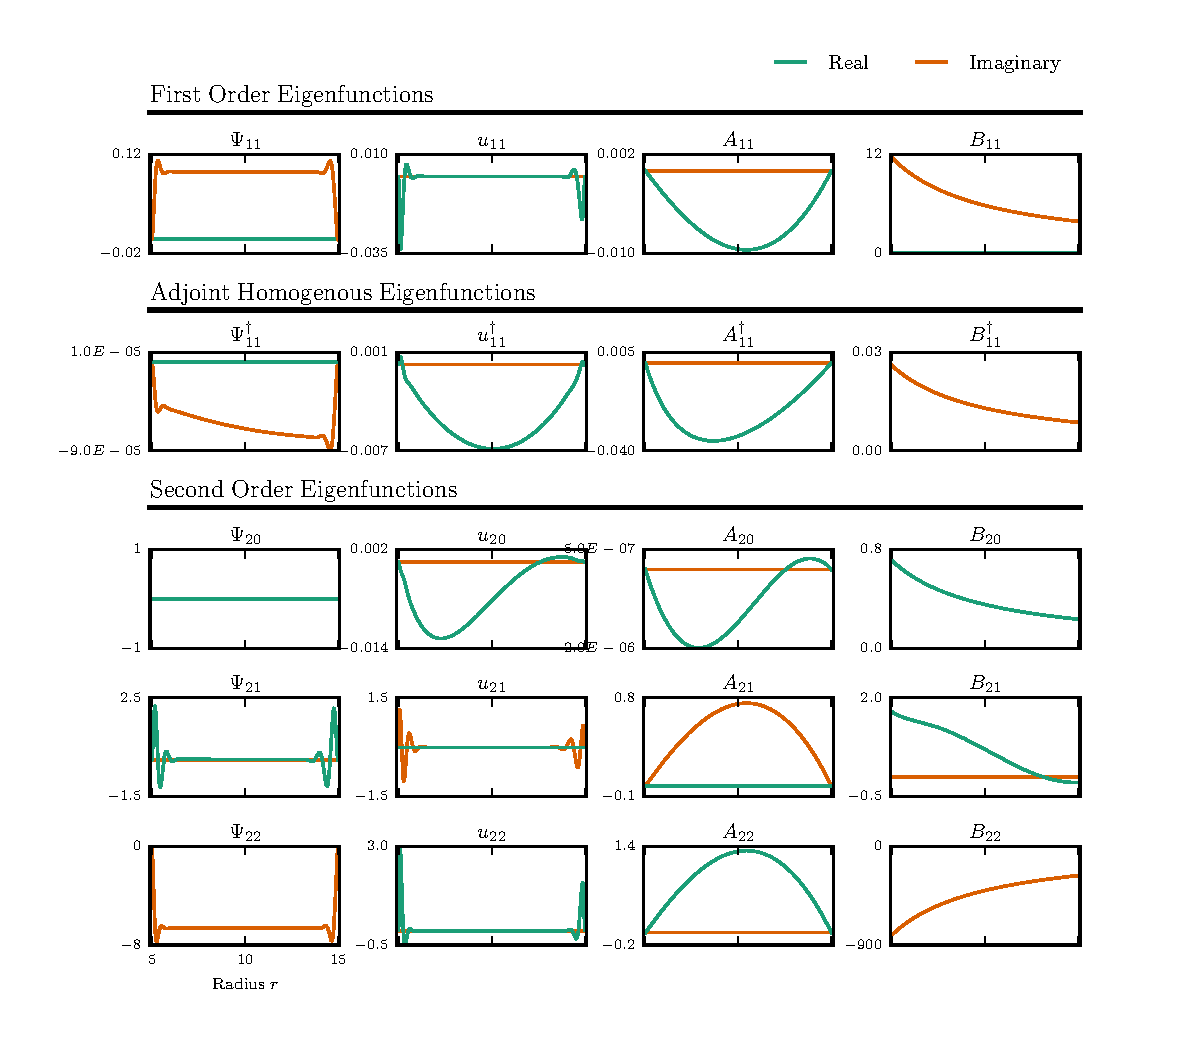
\includegraphics[width=\textwidth]{../python/widegap/figures/orders_1_2_widegap_fiducial_eigenfunctions.pdf}
\caption{Eigenfunctions of the first order equations, first order adjoint homogenous equations, and second order equations. We use our fiducial parameters for the standard MRI ($\xi = 0$). Eigenfunctions are normalized such that either the real or imaginary part is zero.}
\end{figure}

\begin{figure}
\centering
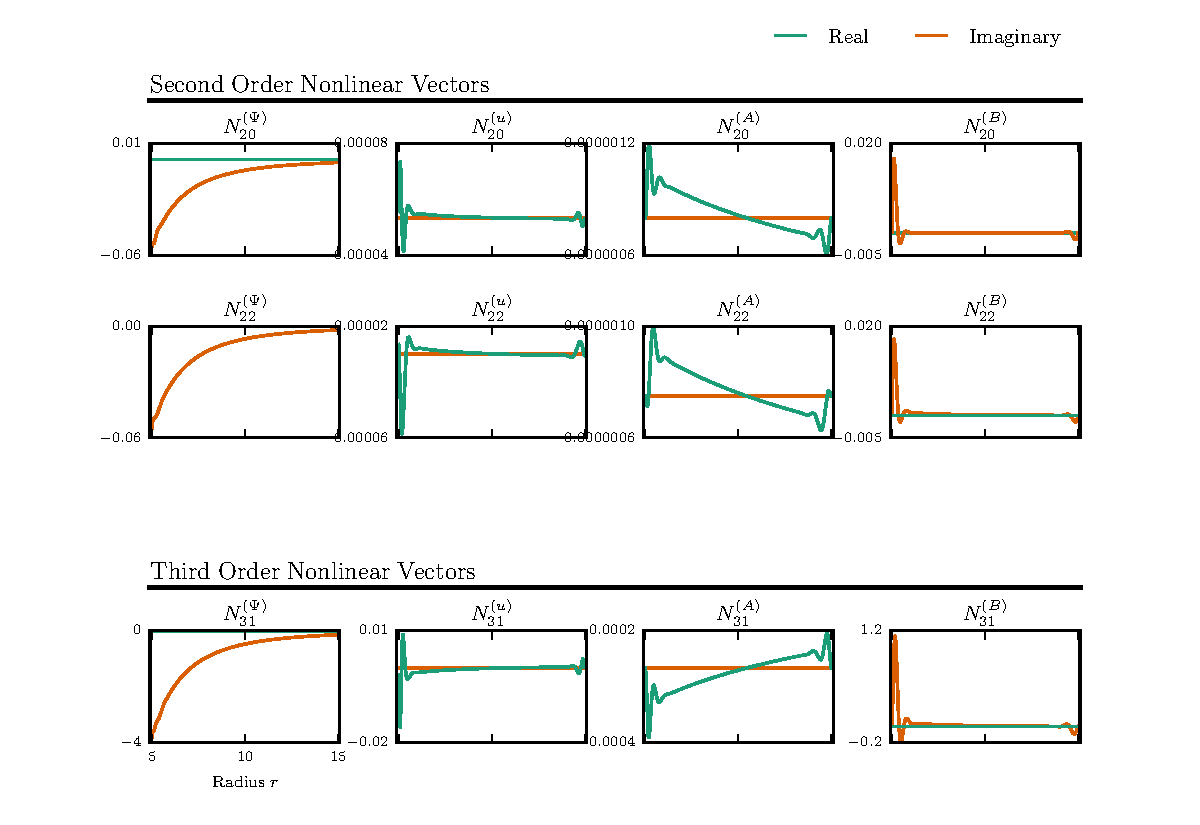
\includegraphics[width=\textwidth]{../python/widegap/figures/nonlinear_2_3_widegap_fiducial_eigenfunctions.pdf}
\caption{Nonlinear terms $N_2$ and $N_3$ for our fiducial standard MRI parameters.}
\end{figure}

See Appendix \ref{app:basic_equations} for the definition of matrices and nonlinear vectors, and a thorough derivation. We emphasize that Equations \ref{eq:ordere} - \ref{eq:ordere3} have the same form as these equations in the narrow gap case, although the matrices (which contain all radial derivatives) are significantly different in this wide gap formulation. This is because we do not have slow variation in the radial dimension. The slow variation in $Z$ and $T$ are parameterized as an amplitude function $\alpha(Z, T)$ which modulates the flow in these dimensions. This parameterization coupled with the boundary conditions lead us to an ansatz linear solution $\mathbf{V}_1 = \alpha(Z, T) \mathbb{V}_{11}(r) e^{i k_z z} + c.c.$, where the radial variation is contained in $\mathbb{V}_{11}$. We defer full expressions and derivations thereof to the Appendix, and focus here on features of the wide gap system which distinguish it from the thin gap limit.

First, the result of the weakly nonlinear analysis is a single amplitude equation for $\alpha$. We find

\beq
 \label{eq:gle}
\partial_T \alpha = b \alpha + d \partial_Z^2 \alpha - c \alpha \left|\alpha^2\right|,
\eeq

a Ginzburg-Landau equation (e.g. \cite{Aranson:2002}). Here we note a departure from the behavior of the thin-gap system. The purely conducting boundary condition states that the axial component of the current ($\mathbf{J}_z = [\nabla \times \mathbf{B}]_z)$ must be zero at the walls. In the thin gap geometry, the purely conducting boundary condition on the azimuthal magnetic field is $\partial_x(B_y) = 0$ for axisymmetric perturbations. A spatially constant azimuthal field satisfies both the thin-gap MRI equations and this boundary condition. This neutral mode is formally included in the analysis of \citei{Umurhan:2007hs} and yields a second amplitude equation in the form of a simple diffusion equation. This amplitude equation decouples from the GLE because of the translational symmetry of the thin-gap geometry. Because that symmetry is not preserved in the wide-gap case, \citeauthor{Umurhan:2007hs} postulate that slow variation in the wide-gap geometry will be governed by two coupled amplitude equations. However, the wide-gap conducting boundary condition $J_z = \frac{1}{r} \partial_r (r B_\phi) = 0$, together with the purely geometric term in Equation \ref{eq:Bphi_perturbed}, conspire to prevent the wide-gap geometry from sustaining a neutral mode. We note that a neutral mode of the form $B_\phi(r) \propto \frac{1}{r}$ would exist in a resistance-free approximation.

The preservation of symmetries in the thin-gap geometry is worth a closer look, as its absence in the wide gap case is the source of many differences in the systems. \citei{Latter:2015} point out that in the ideal limit ($\nu, \eta \rightarrow 0$), the linearized system described by the lefthand side of Equations \ref{eq:Psi_perturbed} - \ref{eq:Bphi_perturbed} can be expressed as a Shr{\"o}dinger equation for the radial velocity. Similarly combining equations to obtain a single expression for $\Psi$, we find that the thin-gap limit linear ideal MRI can be expressed as

\beq
\partial_x^2 \Psi + k_z^2 \mathrm{U}(x) \Psi = 0
\eeq 

where $\mathrm{U}(x) = {3}/{v_A^2 k_z^2} + 1$ at marginality. When no-slip radial boundary conditions are applied, the thin-gap MRI system resembles a particle in a box with a radially constant potential well. Thus thin-gap linear MRI modes must be eigenstates of parity. These symmetries are preserved in the nonlinear MRI terms because they are nonlinear combinations of lower-order eigenfunctions. In the wide gap case, the ``potential" $\mathrm{U}(r)$ varies with $r$, so symmetric and antisymmetric modes are no longer required.

The nonlinear terms, detailed in Appendix \ref{app:nonlinear_terms}, represent an interesting departure from the thin-gap theory. The thin-gap nonlinear terms at both second and third orders are linear combinations of Jacobians. The nonlinear terms in the wide-gap case differ from their thin-gap analogues with in the addition of vertical advective terms. These terms derive from the advective derivatives in the momentum and induction equations, but are filtered out in the thin-gap approximation. These advective terms allow the nonlinear contributions at both second and third order (i.e. N$_2$ and N$_3$) not to individually satisfy the boundary conditions on $\Psi$ and $u$. (I'm just guessing but this may lead to higher torque on inner cylinder -- should calculate) 

\section{Channel Modes}
Channel modes are radially independent linear MRI modes which are, under certain conditions, exact nonlinear solutions to the MRI equations. 

\clearpage
\appendix

\section{A. Detailed Equations}\label{app:basic_equations}

Here we detail the perturbation analysis described in Section \ref{sec:wnl_analysis}. The linear system is described by Equation \ref{eq:unperturbed_matrix_eqns}, where 

\beq
\mathcal{L} = \mathcal{L}_0 + \mathcal{L}_1 \partial_z + \mathcal{L}_2 \partial_z^2 + \mathcal{L}_3 \partial_z^3 + \mathcal{L}_4 \partial_z^4,
\eeq

\beq
\widetilde{\mathcal{G}} = - \mathcal{G} \partial_z - \mathcal{L}_3 \partial_z^3,
\eeq

\beq
\widetilde{\mathcal{H}} = \mathcal{H} \partial_z,
\eeq

and the constituent matrices are defined as 

\beq
\mathcal{L}_0 = \left[\begin{matrix}
-\frac{1}{\reye} (-\frac{3}{r^4} \partial_r + \frac{3}{r^3}\partial_r^2 - \frac{2}{r^2}\partial_r^3 + \frac{1}{r}\partial_r^4) & 0 & 0 & 0 \\
0 & -\frac{1}{\reye} (\partial_r^2 + \frac{1}{r}\partial_r - \frac{1}{r^2}) & 0 & 0 \\
0 & 0 & -\frac{1}{\reym} (\partial_r^2 - \frac{1}{r} \partial_r) & 0 \\
0 & 0 & 0 & -\frac{1}{\reym} (\partial_r^2 + \frac{1}{r}\partial_r - \frac{1}{r^2}) \\
\end{matrix}\right]
\eeq

\beq
\mathcal{L}_1 = \left[\begin{matrix}
0 & -\frac{2}{r} u_0 & \frac{2}{\beta} (\frac{1}{r^2} \partial_r - \frac{1}{r}\partial_r^2) & 0 \\
\frac{1}{r^2} u_0 + \frac{1}{r}\partial_r u_0 & 0 & 0 & -\frac{2}{\beta} \\
-1 & 0 & 0 & 0 \\
0 & -1 & \frac{1}{r^2} u_0 - \frac{1}{r} \partial_r u_0 & 0 \\
\end{matrix}\right]
\eeq


\beq
\mathcal{L}_2 = \left[\begin{matrix}
-\frac{1}{\reye} (-\frac{2}{r^2}\partial_r + \frac{2}{r}\partial_r^2) & 0 & 0 & 0 \\
0 & -\frac{1}{\reye} & 0 & 0 \\
0 & 0 & -\frac{1}{\reym} & 0 \\
0 & 0 & 0 & -\frac{1}{\reym} \\
\end{matrix}\right]
\eeq

\beq
\mathcal{L}_3 = \left[\begin{matrix}
0 & 0 & -\frac{2}{\beta}\frac{1}{r} & 0 \\
0 & 0 & 0 & 0 \\
0 & 0 & 0 & 0 \\
0 & 0 & 0 & 0 \\
\end{matrix}\right]
\eeq

\beq
\mathcal{L}_4 = \left[\begin{matrix}
-\frac{1}{\reye}\frac{1}{r} & 0 & 0 & 0 \\
0 & 0 & 0 & 0 \\
0 & 0 & 0 & 0 \\
0 & 0 & 0 & 0 \\
\end{matrix}\right]
\eeq

\beq
\mathcal{G} = \left[\begin{matrix}
0 & 0 & \frac{2}{\beta}(\frac{1}{r^2}\partial_r - \frac{1}{r}\partial_r^2) & 0 \\
0 & 0 & 0 & -\frac{2}{\beta} \\
-1 & 0 & 0 & 0 \\
0 & -1 & 0 & 0 \\
\end{matrix}\right]
\eeq

\beq
\mathcal{H} = \left[\begin{matrix}
0 & 0 & 0 & \frac{2}{\beta} \frac{2}{r^2} \\
0 & 0 & 0 & 0 \\
0 & 0 & 0 & 0 \\
-\frac{2}{r^3} & 0 & 0 & 0 \\
\end{matrix}\right]
\eeq

\beq
\mathcal{D} = \left[\begin{matrix}
\frac{1}{r}\partial_r^2 + \frac{1}{r}\partial_z^2 - \frac{1}{r^2}\partial_r & 0 & 0 & 0 \\
0 & 1 & 0 & 0 \\
0 & 0 & 1 & 0 \\
0 & 0 & 0 & 1 \\
\end{matrix}\right]
\eeq

\section{B. Nonlinear Terms}\label{app:nonlinear_terms}

Here we detail the perturbative expansion of the nonlinear vector $\mathbf{N}$ in Equation \ref{eq:unperturbed_matrix_eqns}. 

\beq
\mathbf{N} = \epsilon^2 \mathbf{N}_2 + \epsilon^3 \mathbf{N}_3
\eeq

\beq
N_2^{\Psi}  = J(\Psi_1, \frac{1}{r^2} \nabla^2 \Psi_1) + J(\Psi_1, -\frac{2}{r^3}\partial_r\Psi_1)
- \frac{2}{\beta} J (A_1, \frac{1}{r^2} \nabla^2 A_1) - \frac{2}{\beta} J(A_1, -\frac{2}{r^3} \partial_r A_1) - \frac{2}{r} u_1 \partial_z u_1 + \frac{2}{\beta} \frac{2}{r} B_1 \partial_z B_1
\eeq

\beq
\begin{split}
N_2^{u} = \frac{1}{r} J\left(\Psi_1, u_1\right) - \frac{1}{r} \frac{2}{\beta} J\left(A_1, B_1\right) + \frac{1}{r^2} u_1 \partial_z \Psi_1 - \frac{2}{\beta}\frac{1}{r^2} B_1 \partial_z A_1
\end{split}
\eeq

\beq
N_2^A = -\frac{1}{r} J\left(A_1, \Psi_1\right)
\eeq

\beq
N_2^B = -\frac{1}{r} J\left(A_1, u_1\right) - \frac{1}{r} J\left(B_1, \Psi_1\right) - \frac{1}{r^2} B_1 \partial_z \Psi_1 + \frac{1}{r^2} u_1 \partial_z A_1
\eeq

\beq
\begin{split}
N_3^{\Psi} & = J(\Psi_1, \frac{1}{r^2} \nabla^2 \Psi_2) + J(\Psi_2, \frac{1}{r^2} \nabla^2\Psi_1) + 2 J (\Psi_1, \frac{1}{r^2}\partial_Z\partial_z \Psi_1) + J(\Psi_1, -\frac{2}{r^3}\partial_r \Psi_2) + J(\Psi_2, -\frac{2}{r^3}\partial_r \Psi_1) \\
& + \widetilde{J}(\Psi_1, \frac{1}{r^2} \nabla^2 \Psi_1) + \widetilde{J} (\Psi_1, -\frac{2}{r^3}\partial_r \Psi_1) - \frac{2}{\beta} J(A_1, \frac{1}{r^2}\nabla^2 A_2) - \frac{2}{\beta} J(A_2, \frac{1}{r^2}\nabla^2 A_1) - \frac{4}{\beta} J(A_1, \frac{1}{r^2}\partial_Z\partial_z A_1) \\ & - \frac{2}{\beta} J(A_1, -\frac{2}{r^3} \partial_r A_2 ) 
 - \frac{2}{\beta} J(A_2, -\frac{2}{r^3} \partial_r A_1) - \frac{2}{\beta} \widetilde{J} (A_1, \frac{1}{r^2} \nabla^2 A_1) - \frac{2}{\beta} \widetilde{J} (A_1, -\frac{2}{r^3} \partial_r A_1) \\
& - \frac{2}{r} u_1 \partial_z u_2 - \frac{2}{r} u_2 \partial_z u_1 - \frac{2}{r} u_1 \partial_Z u_1 + \frac{2}{\beta}\frac{2}{r} B_1\partial_z B_2 + \frac{2}{\beta}\frac{2}{r} B_2 \partial_z B_1 + \frac{2}{\beta} \frac{2}{r} B_1 \partial_Z B_1
\end{split}
\eeq

\beq
\begin{split}
N_3^u & = \frac{1}{r}J\left(\Psi_1, u_2\right) + \frac{1}{r}J\left(\Psi_2, u_1\right) + \frac{1}{r}\widetilde{J} \left(\Psi_1, u_1\right) - \frac{1}{r}\frac{2}{\beta} J\left(A_1, B_2\right) - \frac{1}{r} \frac{2}{\beta} J\left(A_2, B_1\right) - \frac{1}{r}\frac{2}{\beta}\widetilde{J}\left(A_1, B_1\right) \\
& + \frac{1}{r^2} u_1\partial_z \Psi_2 + \frac{1}{r^2} u_2 \partial_z \Psi_1 + \frac{1}{r^2} u_1 \partial_Z \Psi_1 - \frac{2}{\beta} \frac{1}{r^2} B_1 \partial_z A_2 - \frac{2}{\beta} \frac{1}{r^2} B_2 \partial_z A_1 - \frac{2}{\beta} \frac{1}{r^2} B_1 \partial_Z A_1
\end{split}
\eeq

\beq
N_3^A = -\frac{1}{r} J\left(A_1, \Psi_2\right) - \frac{1}{r}J\left(A_2, \Psi_1\right) - \frac{1}{r} \widetilde{J}\left(A_1, \Psi_1\right)
\eeq

\beq
\begin{split}
N_3^B & = - \frac{1}{r} J\left(A_1, u_2\right) - \frac{1}{r} J\left(A_2, u_1\right) - \frac{1}{r}\widetilde{J}\left(A_1, u_1\right) - \frac{1}{r} J\left(B_1, \Psi_2\right) - \frac{1}{r} J\left(B_2, \Psi_1\right) - \frac{1}{r} \widetilde{J} \left(B_1, u_1\right) \\ & - \frac{1}{r^2} B_1\partial_z \Psi_2 - \frac{1}{r^2} B_2 \partial_z \Psi_1 - \frac{1}{r^2} B_1 \partial_Z \Psi_1 + \frac{1}{r^2} u_1 \partial_z A_2 + \frac{1}{r^2} u_2 \partial_z A_1 + \frac{1}{r^2} u_1 \partial_Z A_1
\end{split}
\eeq


\bibliographystyle{plain}

\begin{thebibliography}{53}
\expandafter\ifx\csname natexlab\endcsname\relax\def\natexlab#1{#1}\fi

\bibitem[{Aranson \& Kramer(2002)}]{Aranson:2002}
Aranson, I.S. \& Kramer, L., 2002, Rev. Mod. Phys. 74, 99

\bibitem[{Clark \& Oishi(2016a)}]{Clark:2016}
Clark, S.E. and Oishi, J.S., 2016, in prep

\bibitem[{Goodman \& Ji(2002)}]{Goodman:2002ix}
Goodman, J. \& Ji, H., 2002, JFM, 462, 365

\bibitem[{Hollerbach \& R\"udiger(2005)}]{Hollerbach:2005tr}
Hollerbach, R. \& R\"udiger, G., 2005, Phys. Rev. Lett. 95, 124501

\bibitem[{Kirillov \& Stefani(2013)}]{Kirillov:2013}
Kirillov, O, \& Stefani, F, 2013, Phys. Rev. Lett. 111, 061103

\bibitem[{Latter et al.(2015)}]{Latter:2015}
Latter, H.N., Fromang, S., \& Faure, J., 2015, MNRAS 453, 3257

\bibitem[{Liu et al.(2006)}]{Liu:2006}
Liu, W, Goodman, J, Herron, I, and Ji, H, 2006, Phys. Rev. E 74, 056302

\bibitem[{R\"udiger \& Hollerbach(2007)}]{Rudiger:2007}
R\"udiger, G, \& Hollerbach, R, Phys. Rev. E 76, 068301

\bibitem[{Stefani et al.(2006)}]{Stefani:2006iv}
Stefani, F, Gundrum, T, Gerbeth, G, R\"udiger, G, Schultz, M, Szklarski, J, Hollerbach, R, Phys Rev Lett, 2006, 97, 184502

\bibitem[{Stefani et al.(2009)}]{Stefani:2009hp}
Stefani, F, Gerbeth, G, Gundrum, T, Hollerbach, R, Priede, J, R\"udiger, G, and Szklarski, J, Phys Rev E, 80, 066303

\bibitem[{Umurhan et al.(2007a)}]{Umurhan:2007dz}
Umurhan, O.M., Regev, O., Menou, K., 2007, Phys. Rev. Letters, 98, 034501

\bibitem[{Umurhan et al.(2007b)}]{Umurhan:2007hs}
Umurhan, O.M., Regev, O., Menou, K., 2007, Phys. Rev. E, 76, 036310


\end{thebibliography}

\end{document}

